\section{Battery Management System}
The purpose of the BMS is to observe and make sure that the propulsion battery is kept within a safe operation area at all times. It does this by monitoring cell voltages, temperature and current from the battery. The data the BMS collects from these units is compared to lower and upper threshold limits that are in compliance with the requirements from the Shell Eco-Marathon committee \footnote{See "sem-2016-global-rules-chapter1-010715"}. In case an event occurs where the temperature, cell voltages or current from the battery exceed the allowed thresholds, then the BMS must autonomously make sure to protect the rest of the vehicle from over-current by isolating the battery. \\
The BMS is designed to be as low power consuming as possible

\begin{figure}[H]
	\centering
	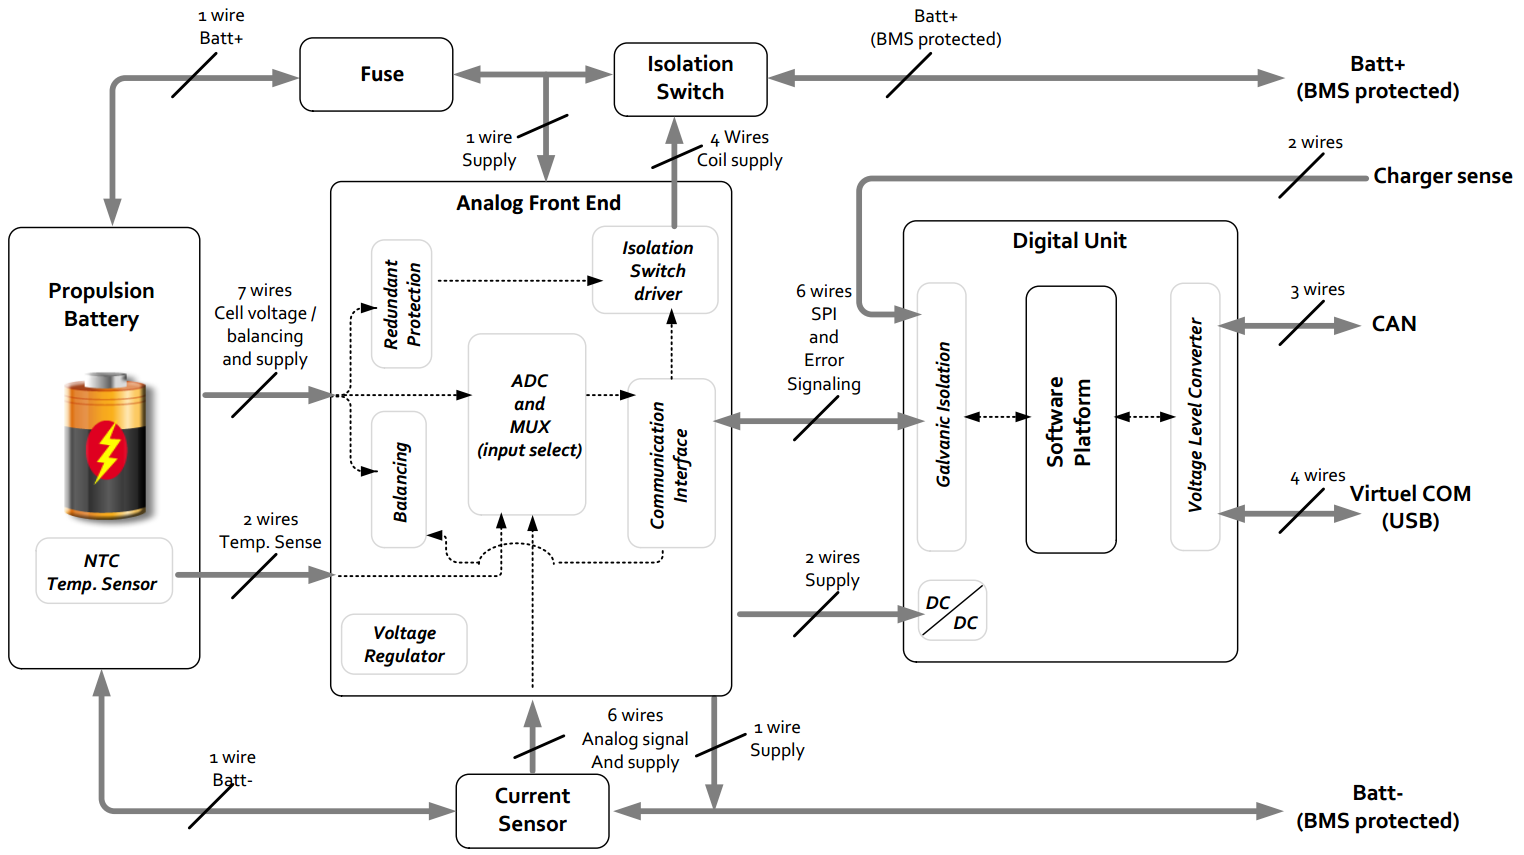
\includegraphics[width=1.0\linewidth]{Hardware/Pictures/BMSOverview}
	\caption[Empty]{An elaborated system and interfacing diagram for the BMS\footnotemark}
	\label{fig:BMSOverview}
\end{figure}
\footnotetext{Reference to 2013BMS\fxnote{Reference to 2013BMS Documentation sec 2.4}}



INTRO HERE ------\\
Batteri besparelse -- lav strøms stilstand (quiescent)... from for færdig solution... State of BMS...
Hardware overview \\ 

\ref{fig:IBD_BMS}



\subsection{Disclaimer}
In this chapter a detailed documentation of the BMS' hardware will be given. Furthermore, each unit contained in the BMS will be described where the implementation and contents of each unit's circuitry is viewed upon as a black-box. This means that the units will be considered purchased from a third party vendor and therefore a detailed description of the circuitry will not be given. This will lead to a different form of documentation with a lot of references to the "manufacturer's" documentation that is the "BAC-projekt\_BMSogbatteri\_2013", which was done by Jonas Nyborg in 2013. \fxnote{Reference to 2013BMS Documentation} documentation.
Thus the general purpose and overview of each unit will elaborated in this chapter. 

\subsubsection{Propulsion battery}
Er flyttet til Hardware/Battery \fxnote{Delete later}

\subsection{Analog Front end}
The purpose of this unit is that it performs calculations and analog to digital conversion of the battery's cell voltages, battery's temperature and the signal from current sensor. Moreover, this unit manages cell balancing on request from the digital unit. It also has additional battery protection independent of the digital unit.
An overview of the Analog Front End can be seen on figure \ref{fig:frontendOverview}.

\begin{figure}[H]
	\centering
	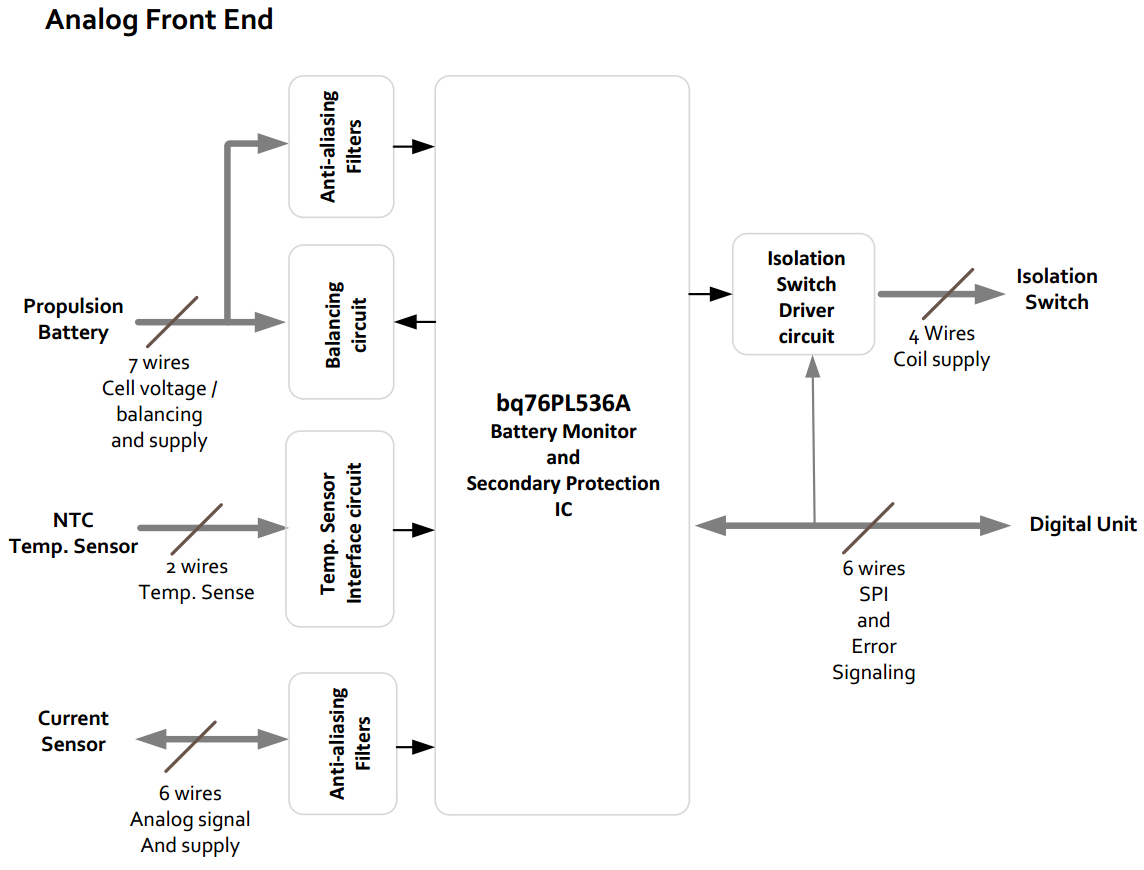
\includegraphics[width=1.0\linewidth]{Hardware/Pictures/analogfrontendOverview}
	\caption[Empty]{Analog Front End circuit blocks\footnotemark}
	\label{fig:frontendOverview}
\end{figure}
\footnotetext{Reference to 2013BMS\fxnote{Reference to 2013BMS Documentation}}

Now every circuit block will be elaborated on its functionality and how it all works. If you wish to receive an even more thorough and detailed explanation, calculations and choices for components included, on the Analog Front End please see the \fxnote{reference to BMS2013 documentation}\\

\subsubsection{Anti-aliasing filters and cell balancing}
The anti-aliasing filters are there to decrease unwanted AC noise and they're placed very near their respective ADC inputs. The filters are traditional 1. order RC low-pass filters and they are implemented with respects to the battery monitor IC, which will be discussed in a moment.\\
The balancing circuit is connected to the battery monitor IC where it has outputs that are capable of controlling balancing of the cells. This process can be initialized by the Digital Unit if given parameters exceed a specific threshold. The circuit can charge the cells  when it is connected to a charger to balance them by discharging them into bleeder resistors located on the circuit. This is done to keep the cells within the recommended safe operation area, which is in between 3-4.2V.

\subsubsection{Battery Monitor IC}
The heart of the BMS is the bq76PL536A-Q1 Battery Monitoring IC (new chip used since 2014 instead of the one on figure \ref{fig:frontendOverview}). It was chosen as it offers very low quiescent current, secondary protection, high precision voltage measurements and has the choice of stacking several IC's to attain support of a respective number of cells. The core functionality of this said chip is that it can receive and handle a lot of commands at the same time. As you see on figure \ref{fig:frontendOverview} it is connected to several circuits. It's job is, among other things, to receive a vast amount of data from it's surroundings / connected circuits. Example of data could be data requests from the Digital Unit, cell voltages, current sensor signal, cell temperature signal balancing requests from the Digital unit and more. With all of this data the Battery Monitoring IC converts this data through its ADC's where it sends them off to the Digital Unit. It can also perform the balancing if it receives a request. Furthermore, it is possible for it to drive the Isolation Switch, which means that in an event where the safe operation area is exceeded, it can cut off the power from the battery supply to the rest of the vehicle.

\subsubsection{Temperature sensor}
\fxnote{Evt. lave referencer til hvert eneste kapitel i BMS, ellers bare referere til et stort afsnit i starten også lade det være det. Også selvfølgelig referere billeder og ting taget fra rapporten.}
The temperature sensor is rather self explanatory, its purpose is to measure the temperature of the batteries. To do this a Thermistor(NTC) has been used to get voltage readouts by converting the temperature from the Thermistor. The temperature thresholds are specified in AU2\_F14, which can be seen here: \ref{sec:requirements}. If the given threshold is exceeded the Isolation Switch will prevent current from flowing through it.

\subsubsection{Isolation Switch Driver circuit}
The purpose of this part is to assure and allow the Battery Monitor IC and Digital Unit to control the Isolation Switch. In case of a parameter exceeding a threshold this is how the BMS shuts off current to the rest of the vehicle - By using the Isolation Switch Driver circuit.\\

\subsection{Analog Front End: Extension Module}
The Extension Module unit's purpose is that it gives the BMS the capability to support a larger amount of battery cells. Since the BMS Front End only supports 6 cells - and using the Extension Module the BMS can support up to 18 cells. This is done by stacking the Battery Monitor ICs - See figure \ref{fig:BMSextensionmod}. The Extension Module resembles the Analog Front End, however, it doesn't include the same features. Features like SPI to the Digital Unit, current sensor input and Isolation Switch Driver are left out and not included. It's purpose is to communicate with the Battery Monitor IC and report the voltages from the other cells. That way the BMS has full control and is able to monitor all the batteries.\\

\begin{figure}[H]
	\centering
	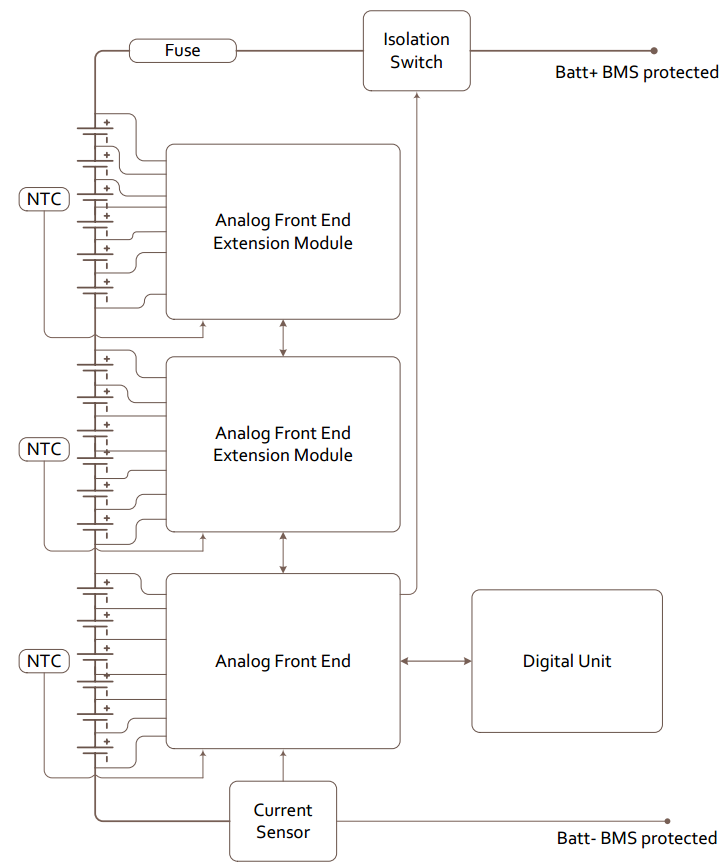
\includegraphics[width=1.0\linewidth]{Hardware/Pictures/BMSextensionmod}
	\caption[Empty]{Connection of Extension Modules\footnotemark}
	\label{fig:BMSextensionmod}
\end{figure}
\footnotetext{Reference to 2013BMS\fxnote{Reference to 2013BMS Documentation kap 3.1.3}}

On figure \ref{fig:BMSextensionmod} you can see an overview of how a possible stacking of Battery Monitor ICs can be handled. You can also see that only the Analog Front End has a connection to the Digital Unit through SPI.\\
The fuse block seen on figure \ref{fig:BMSextensionmod} is a fast-acting fuse that can handle up to 30A before it breaks. It is implemented as a requirement by the Shell Eco-Marathon committee.\\
A few things to note on this diagram: The extension modules are capable of utilising an NTC Thermistor, however, for simplicity it has been chosen that only the Analog Front End contains and handles the Thermistor to measure the temperature of the batteries. One of these is more than enough since the other Thermistors would simply put out almost or exactly the same readings.\\


\subsection{Current Sensor}
The purpose of this unit is to measure the amount of current flowing through the sensor as well as the direction of the current. The data that the sensor generates is sent to and handled by the Analog Front End. \\
The choice for a current sensor was either to use a Hall current sensor as done in the Motor Controller unit or use a shunt current sensor. Since the goal is to make the BMS as energy efficient as possible the choice fell on the shunt based sensor. It is a better choice when considering the power consumption for the current sensor, more on the specifications and calculations can be found in xx \fxnote{reference BMS 2013 sec 3.1.4}.

\subsection{Isolation Switch}
The Isolation Switch has a very important functionality concerning the BMS. If anything goes wrong with the battery, which means it exceeds the safe operation area of any specified thresholds, then the Isolation Switch will prevent any current from flowing through it and to the distribution block. \\
Since it is a requirement by the Shell Eco-Marathon committee that an automatic form of isolation of the battery from the rest of the system is required within the BMS. This leaves us with the only choice of using a relay to fulfil this requirement. Nonetheless, a relay isn't the best solution when considering low power application and consumption. If the BMS was to be implemented in a commercial application where it wouldn't be obligatory to fulfil the Shell Eco-Marathon committee's requirement, then a solution using RDS MOSFETs would be a huge benefactor when considering supply current draw.\\
The Isolation Switch relay is of a type Normally Open(NO), which means unless it has a specific amount of voltage running through it's coils, then it won't allow current to flow through it's terminals. Nonetheless, the relay is  capable of withstanding a current of up to 30 Amps and has a nominal coil rating of 48V, which is within the specified ratings by Shell's rules. Below on figure \ref{fig:BMSRelay} the physical relay can be seen.

\begin{figure}[H]
	\centering
	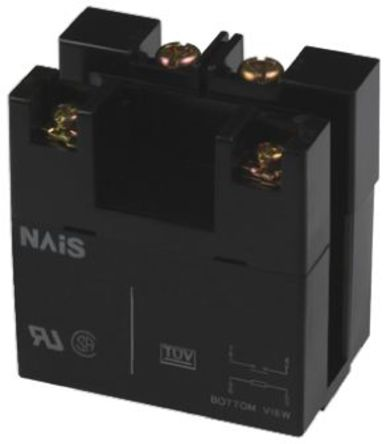
\includegraphics[width=0.3\linewidth]{Hardware/Pictures/BMSRelay}
	\caption[Empty]{Picture of the Isolation Switch Relay used in the BMS\footnotemark}
	\label{fig:BMSRelay}
\end{figure}
\footnotetext{\url{http://uk.rs-online.com/web/p/non-latching-relays/6995676/} (Date: 21-05-2016)}

The Isolation Switch works by having the Digital Unit send commands to the Analog Front End, which in return controls the Isolation Switch Driver. And the driver controls the relay. If the cells are within a safe operation area and the Digital Unit hasn't told the Analog Front End to open the relay - meaning to prevent current flowing through it - then a secondary option is available to isolate the battery manually. This functionality is implemented by a Emergency Switch(button). It serves the purpose of delivering a 0V drop over the relay's coil when the Emergency Switch is pressed. This will force the relay to open and seize to supply current through its terminals and therefore isolate the battery.

\subsection{Digital Unit (HW)}
This unit's purpose is to gather the measured values from the Analog Front End and thereafter run calculations and approximations of cell and battery parameters. If any of these parameters exceeds a specific threshold then the Digital Unit is capable of utilizing the Isolation Switch to prevent damages to the rest of the vehicle's system. The Digital Unit is capable of communication with external units. Furthermore, the Digital Unit utilizes galvanic isolation and a DC/DC converter, which will be described in detail below. 

\begin{figure}[H]
	\centering
	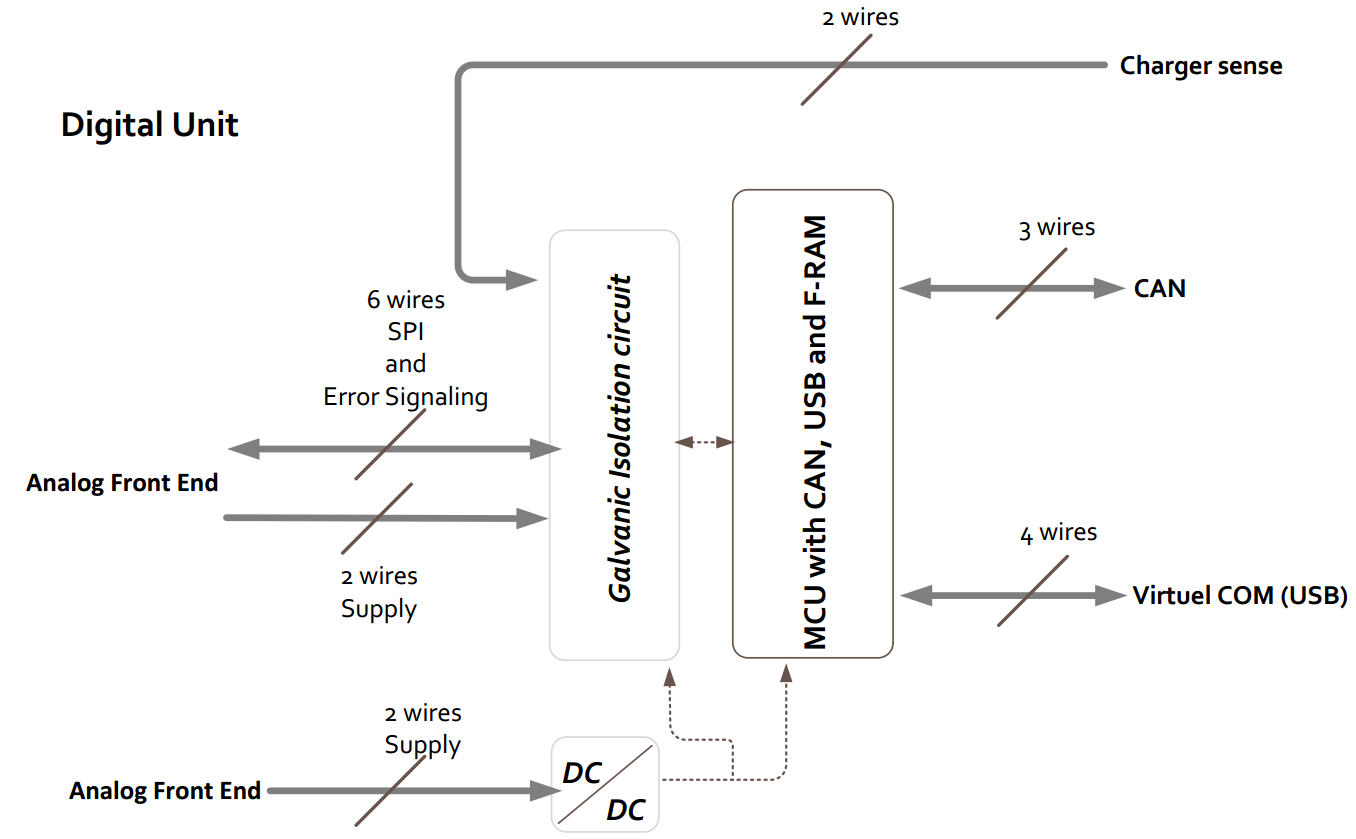
\includegraphics[width=1.0\linewidth]{Hardware/Pictures/BMSdigitalUnit}
	\caption[Empty]{Digital Unit circuit blocks\footnotemark}
	\label{fig:BMSdigitalUnit}
\end{figure}
\footnotetext{Reference to 2013BMS\fxnote{Reference to 2013BMS Documentation kap 3.1.6}}

On figure \ref{fig:BMSdigitalUnit} you can see the Digital Unit and its contents. A elaborative description will be given on each of the circuit blocks in this section. As mentioned earlier none of the implementation will be addressed since this unit along with others are viewed upon as a black box.

\subsubsection{Galvanic Isolation}
Galvanic isolation is a principle of isolating functional parts of electrical systems to prevent flow of current. This means that no direct path of conductivity is permitted. However, information can still be exchanged by utilization of different techniques such as electromagnetic waves or by optical and mechanical means. These are simply a few methods mentioned, there are a lot of various ways to transmit information by using galvanic isolation.\\
In any case, the way the galvanic isolation is used in the BMS is through the use of optocouplers. Optocouplers or opto-isolators are components that by the use of light can transfer electrical signals between two isolated circuits. This application often consists of an LED on the sender side, and a photodiode on the receiver side - You can see figure \ref{fig:BMSoptocoup} for a quick orientation of the principle.

\begin{figure}[H]
	\centering
	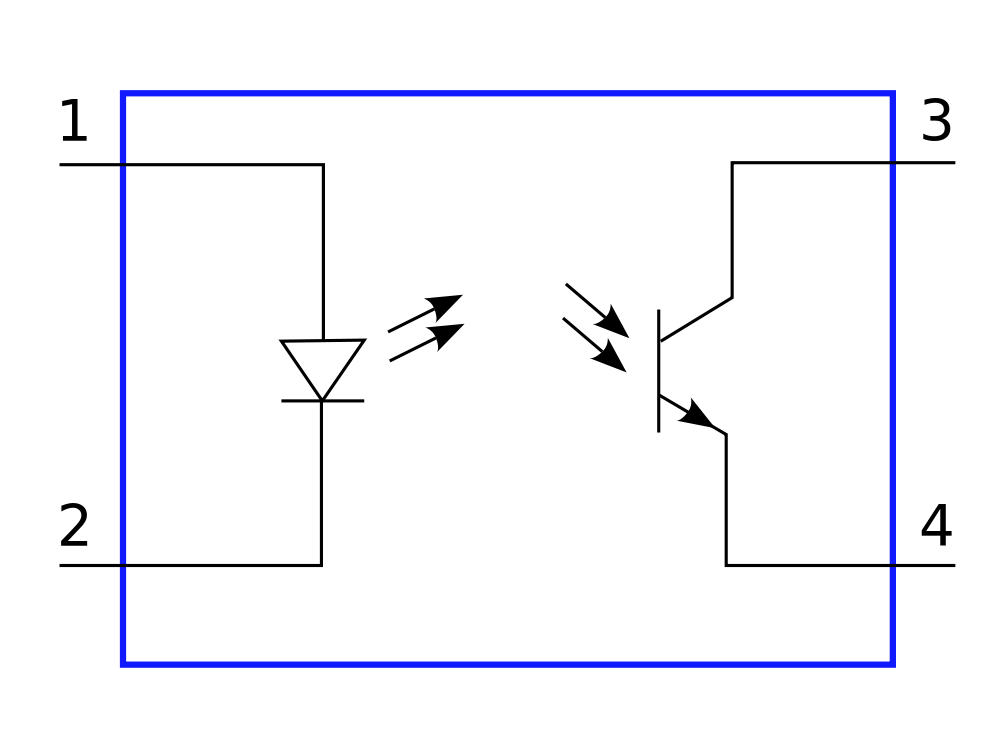
\includegraphics[width=0.5\linewidth]{Hardware/Pictures/BMSoptocoup}
	\caption[Empty]{Basic illustration of the functionality of an optocoupler\footnotemark.}
	\label{fig:BMSoptocoup}
\end{figure}
\footnotetext{\url{https://commons.wikimedia.org/wiki/File:Optocoupler.svg} (Date: 22-05-2016)}

When the sender side wants to send something it activates the LED. The light from the LED activates the photodiode on the other side of the isolated circuit. Then through either OP-AMPs or transistors the light received in the photodiode can be translated into electrical signals and thus you utilize light to send information. Other than being able to send information through light, the optocouplers are also good for safety. They can often withstand high input-to-output voltages and voltage transients. \\
With low power consumption in mind, a few digital isolators based on optocouplers were examined to find the best possible solution. You can see more about which digital isolators were investigated in the \fxnote{reference to BMS2013 sec 3.1.6.1}. The examination of the two digital isolators resulted in neither of them being chosen since they were consuming to much power on both the receiver and sender side. Therefore the Galvanic Isolation circuit is based on dual-channel optocouplers. This design approach makes it possible to have a low power consumption during use and nearly nothing while quiescent. Furthermore, when the SPI bus isn't used for non-isolated devices a smart power saving option has been implemented, more on this can be found in \fxnote{BMS2013 reference cap 3.1.6.1}.

\subsubsection{DC/DC Converter}
The purpose of the DC/DC Converter is to convert the battery voltage, which is expected to be around 44.4V nominal, to a lower voltage that is usable by the other components in the Digital unit. This includes the Galvanic Isolation and micro controller circuit with its included parts. \\
Since power consumption is a very important factor in the design of the BMS, several DC/DC converters were examined to see if it was possible to find a suitable prefabricated and commercial DC/DC converter. The results of this inspection and a more detailed description of the converter can be found in \fxnote{reference to BMS2013 sec 3.1.6.2}. Moreover, please note that a newer DC/DC Converter than in the 2013 BMS Documentation has been used - More details on the changes done since the 2013 documentation can be found in section \fxnote{reference to CHANGES from BMS 2013 to BMS 2014}.  

\subsubsection{MCU with CAN, USB and F-RAM}
This unit is the brains of the operation. It consists of vital parts to make the BMS function properly. It has a micro controller that has an implemented CAN controller. It also has non-volatile memory, which is in the form of Ferroelectric Random Access Memory (F-RAM). Nonetheless, a USB interface is also part of this unit, which makes it possible to directly debug the BMS through the micro controller. For more info on how to use the USB interface and how to program the BMS see section \ref{sec:BMSDebugging}.\\

\textbf{The MCU - AVR-CAN}\\
The micro controller unit is a OLIMEX AVR-CAN development board. It would have been sufficient to have emulated a CAN interface. However, the platform is now equipped for future improvements by using a micro controller with an integrated CAN controller. This way a CAN protocol is required for the BMS if it is to become commercially viable.

\begin{figure}[H]
	\centering
	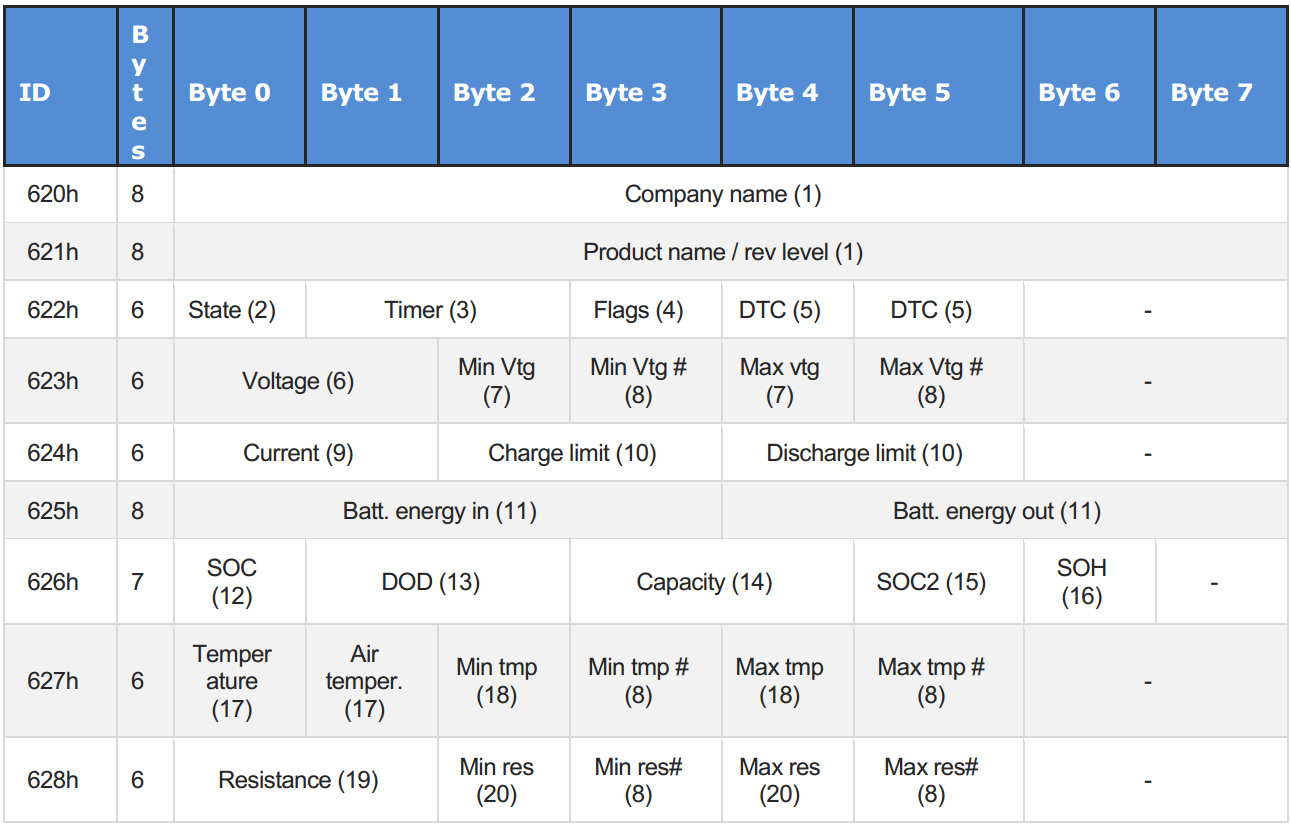
\includegraphics[width=1.0\linewidth]{Hardware/Pictures/BMSCANProto}
	\caption[Empty]{CAN protocol for the BMS\footnotemark}
	\label{fig:BMSCANProto}
\end{figure}
\footnotetext{Reference to 2013BMS\fxnote{Reference to 2013BMS Documentation kap 1.5.3.1}}

On figure \ref{fig:BMSCANProto} you can see the CAN protocol, which is based on the Original Standard Traction Pack. Since the BMS was first implemented with a CAN bus it was found that it would be a good idea to perform heavy duty data logging on the Motor Controller via CAN bus, therefore a CAN transceiver and software to support it was implemented on the Motor Controller. For more info about the Can-transceiver see section \ref{sec:CAN-Tranceiver}. A more detailed description of the CAN protocol can be found in \fxnote{reference to BMS2013}.\\
Otherwise the AVR-CAN is mainly used as a control unit, since it performs calculations and sends commands to the Analog Front End all whilst monitoring different thresholds for safe operation areas for the batteries. The AVR-CAN is mainly used for programming and this is where all the BMS Software is stored and executed by the AT90CAN128 IC which is contained on the developer board. The software functionality will be described in the BMS Software chapter \fxnote{Godt med krydsreferencer til forskellige dokumenter - burde være include(xr) ... ?} %\externaldocument{BMSSoftware}.. 

\textbf{F-RAM}\\
As mentioned earlier it was required by the 2013 requirements (BMS\_F.5)\fxnote{reference BMS 2013 sec 1.5.1.2.} that the BMS must be able to store the most critical information on internal memory for the ability to read the data on the USB interface or SD-card on the Motor Controller. Since the AVR-CAN module didn't have enough on-board memory a few options were considered for implementing a solution. EEPROM was considered since it is non-volatile and cheap but offers a limited amount of write cycles as well as the power consumption is fairly higher than the  F-RAM. However, the solution is F-RAM, which is non-volatile has a lot of write cycles and is fairly low power between write cycles. Moreover, please note that a newer F-RAM module than in the 2013 BMS Documentation has been used - More details on the changes done since the 2013 documentation can be found in section \fxnote{reference to CHANGES from BMS 2013 to BMS 2014}.  


%\subsection{Implementation}
%\subsection{Unity test}

\subsection{Programming Quick Guide}
\label{sec:BMSDebugging}
The purpose of this section is meant to help whoever is going to work with the BMS in the future. Here you will be guided in how to use, debug and program the Digital Unit thus the BMS.

Firstly, you will need a few prerequisites listed below to be able to program the BMS. Since the BMS was originally build in 2013 the software to program the BMS is outdated but sometimes it is only possible to proceed and get it to work with the specified utilities. 

Tools required to program the BMS are listed here:
	\begin{itemize}
		\item AVR Studio 4 (tested with version 4.19 Build 730).
		\item Atmel Studio 6 or 7 (Both tested).
		\item JTAG-USB programmer (programmer that is included with the BMS hardware).
		\item 2 batteries (used to power the BMS).
		\item Tera Term (or any other hyper terminal).
		\item USB-A to USB mini cable (used to debug the BMS and see readouts from Tera Term).
	\end{itemize}
	
After you have acquired these tools you are ready to proceed. First of you connect the USB cable from your computer to the BMS front end. Then you launch your chosen hyper terminal and select the COM-port which the BMS has. Afterwards you configure the hyper terminal, where the two most important settings are the baud rate and the way you receive from the BMS. Set the baud rate to 38400, 1 stop bit, 8 data bits and 0 parity bits. Then you specify the newline settings so that you receive both CR+LF else select AUTO. In Tera Term you go to Setup->Terminal->New-line to perform these changes. 
Now you can attach the two batteries to the BMS (remember to plug in both the main plug and the cell plug to the front end), once this is done you're ready to receive data from the front end and it should look something like in the figure below \ref{fig:BMSTeraTerm}.
\begin{figure}[H]
	\centering
	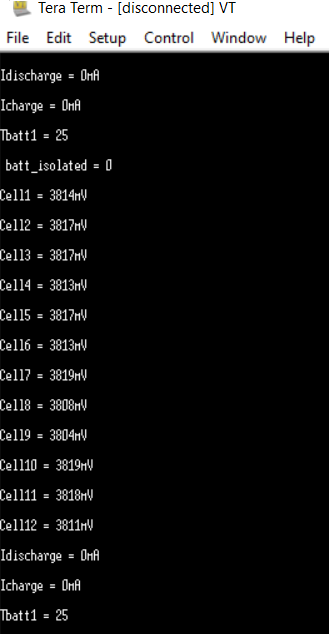
\includegraphics[width=0.6\linewidth]{Hardware/Pictures/BMS_teraterm}
	\caption{Tera Term Printout from BMS}
	\label{fig:BMSTeraTerm}
\end{figure}

Now you're ready to program the BMS. You can compile the code from either Atmel Studio 6 or 7, when you're done compiling you'll have a .hex file which is used for the AVR-CAN (Digital Unit). From this point on you have to follow the guide located in the pdf-file "How-to-install-and-use-AVR-JTAG-USB.pdf" which is located in the BMS repository. Now you can program the AVR-CAN module by selecting the .hex file or other valid files and program the BMS.

You can always confirm the programming by looking at the hyper terminal printouts and see if it matches your expectations. However, if it does not match your expectations you will have to debug the source code or the hardware to resolve the problem.

